\documentclass[a4paper]{article}

\usepackage{xparse}
\usepackage[table, xcdraw, dvipsnames]{xcolor} % Only load xcolor once, with all needed options
\usepackage{colortbl}
\usepackage{circuitikz}
\usepackage{cancel}
\usepackage{siunitx}
\usepackage{float}
\usepackage{multirow}
\usepackage{array}
\usepackage{times}
\usepackage{tikz}
\usepackage[margin=0cm]{geometry}
\usepackage{graphicx}
\usepackage{anyfontsize}
\usepackage{fancyhdr}
\usepackage{indentfirst}
\usepackage{amsmath}
\usepackage[spanish]{babel}
\usepackage[utf8]{inputenc}
\usepackage[explicit]{titlesec}
\usepackage{etoolbox}
\usepackage{multicol}
\usepackage{enumitem}
\usepackage{caption}
\usepackage{subcaption}
\usepackage{booktabs}
\usepackage{amsfonts}
\usepackage[version=4]{mhchem}
\usepackage{lastpage}
\usepackage{hyperref}




\begin{document}
\newcommand{\inicioCodigo}{
    \newpage
    \fancyfoot[C]{}
    \onecolumn
}

\newcommand{\finalCodigo}{
    \newpage
    \fancyfoot[C]{
        \begin{tikzpicture}[remember picture, overlay]
            \draw[gray!30, line width=0.4pt]
                (0cm, 1cm) -- (0cm, 25cm);
        \end{tikzpicture}
    }
    \twocolumn
}

\renewcommand{\theenumi}{\Roman{enumi}}
\definecolor{gold}{rgb}{1.0, 0.84, 0.0}
\newcommand{\resistencia}[4]{
    \begin{minipage}{2cm}
        \begin{center}
            \begin{tikzpicture}
                \draw(-0.4cm, -0.15cm) rectangle (0.4cm, 0.15cm);
                \fill[resistor] (-0.4cm, 0) -- (-0.5cm, 0);
                \draw (-0.4cm, 0) -- (-0.5cm, 0);
                \draw (0.4cm, 0) -- (0.5cm, 0);
                \fill[#1] (-0.35cm, -0.15cm) rectangle (-0.25cm, 0.15cm);
                \fill[#2] (-0.15cm, -0.15cm) rectangle (-0.05cm, 0.15cm);
                \fill[#3] (0.05cm, -0.15cm) rectangle (0.15cm, 0.15cm);
                \fill[#4] (0.25cm, -0.15cm) rectangle (0.35cm, 0.15cm);
            \end{tikzpicture}
        \end{center}
    \end{minipage}
}
\newcommand{\diodoSilicio}[1]{
    \begin{minipage}{2cm}
        \begin{center}
            \begin{circuitikz}[scale=0.5]
                \draw[line width=1pt] (-2,0) -- (-1,0);
                \draw[line width=1pt] (2,0) -- (1,0);

                \filldraw[fill=black!75, draw=black] (-1, -0.5) rectangle (1, 0.5);

                \fill[gray!60] (0.6, -0.5) rectangle (0.8, 0.5);

                \node at (0, -1) {\texttt{#1}};
            \end{circuitikz}
        \end{center}
    \end{minipage}
}
\newcommand{\diodoGermanio}[1]{
    \begin{minipage}{2cm} 
        \begin{center}
            \begin{circuitikz}[scale=0.5]
                \draw[line width=0.8pt] (-2.5,0) -- (-1.5,0);
                \draw[line width=0.8pt] (2.5,0) -- (1.5,0);

                \filldraw[fill=white, draw=black] (-1.5, -0.4) rectangle (1.5, 0.4);
                \fill[orange!80] (-1.5, -0.25) rectangle (1.5, 0.25);
                \fill[gray!95] (1.2, -0.4) rectangle (1.5, 0.4);
                \node at (0, -0.9) {\texttt{#1}};
            \end{circuitikz}
        \end{center}
    \end{minipage}
}
\newcommand{\inv}[1]{\frac{1}{#1}}
\newcommand{\recuadrar}[2]{
    \begin{center}
        \begin{tabular}{|m{#1}|}
            \toprule
            \multicolumn{1}{|c|}{\hspace{5pt}#2\hspace{5pt}} \\
            \bottomrule
        \end{tabular}
    \end{center}
}

\newcommand{\ecuacion}[1]{
    \begin{center}
        $#1$
    \end{center}
}

\newcommand{\longsection}[2]{%
    \section[#1]{\parbox{\columnwidth}{#1}}
}

\newcommand{\saltoPag}[0]{%
    \newpage\noindent\thispagestyle{fancy}%
    \begin{tikzpicture}[remember picture, overlay]
        \draw[line width=0.4pt, color=gray!50] (8.5cm, -0.4cm) -- (8.5cm, -24cm);
    \end{tikzpicture}%
    \ignorespaces{}
}

\newcommand{\midTitle}[2]{%
    \begin{center}
        \textcolor{#1}{\underline{#2}} 
    \end{center}
}

\captionsetup{
    format=hang,
    labelfont={bf},
    textfont=normalfont,
    labelsep=colon,
    justification=centering,
    singlelinecheck=true
}

\newcommand{\imagen}[3][]{
    \begin{center}
        \begin{tikzpicture}
            \node[inner sep=2pt] (image) {\includegraphics[width=#2]{#3}};
            \draw[line width=1pt, color={rgb:red,251;green,73;blue,52}] (image.south west) rectangle (image.north east);
        \end{tikzpicture}
        \ifx\\#1\\
            \captionof{figure}{}
        \else
            \captionof{figure}{#1}
        \fi 
        \label{fig:#2}
    \end{center}
}

\newcommand{\sangria}[0]{\par\noindent\hspace*{15pt}}

\newcommand{\longsubsection}[2]{%
    \subsection[#1]{\parbox{\columnwidth}{#1}}%
}
\author{}\date{}\title{}
\thispagestyle{empty}
\begin{tikzpicture}[remember picture, overlay]
    \pgftransformshift{\pgfpoint{0cm}{0cm}}
    \draw [line width=2pt](1cm,-1cm) -- (1cm,-27.7cm) -- (14cm, -27.7cm) -- (14cm, -1cm) -- (1cm, -1cm);
    \draw[line width=2pt] (15cm, -27.7cm) -- (19cm,-27.7cm) -- (19cm, -1cm) -- (15cm, -1cm) --  (15cm, -27.7cm);
    \node [line width=2pt] at (17cm, -3.5cm) {
\includegraphics[width=3cm]{./imagenes/utn.png}};
	\node [line width=2pt] at (7.5cm, -9cm) {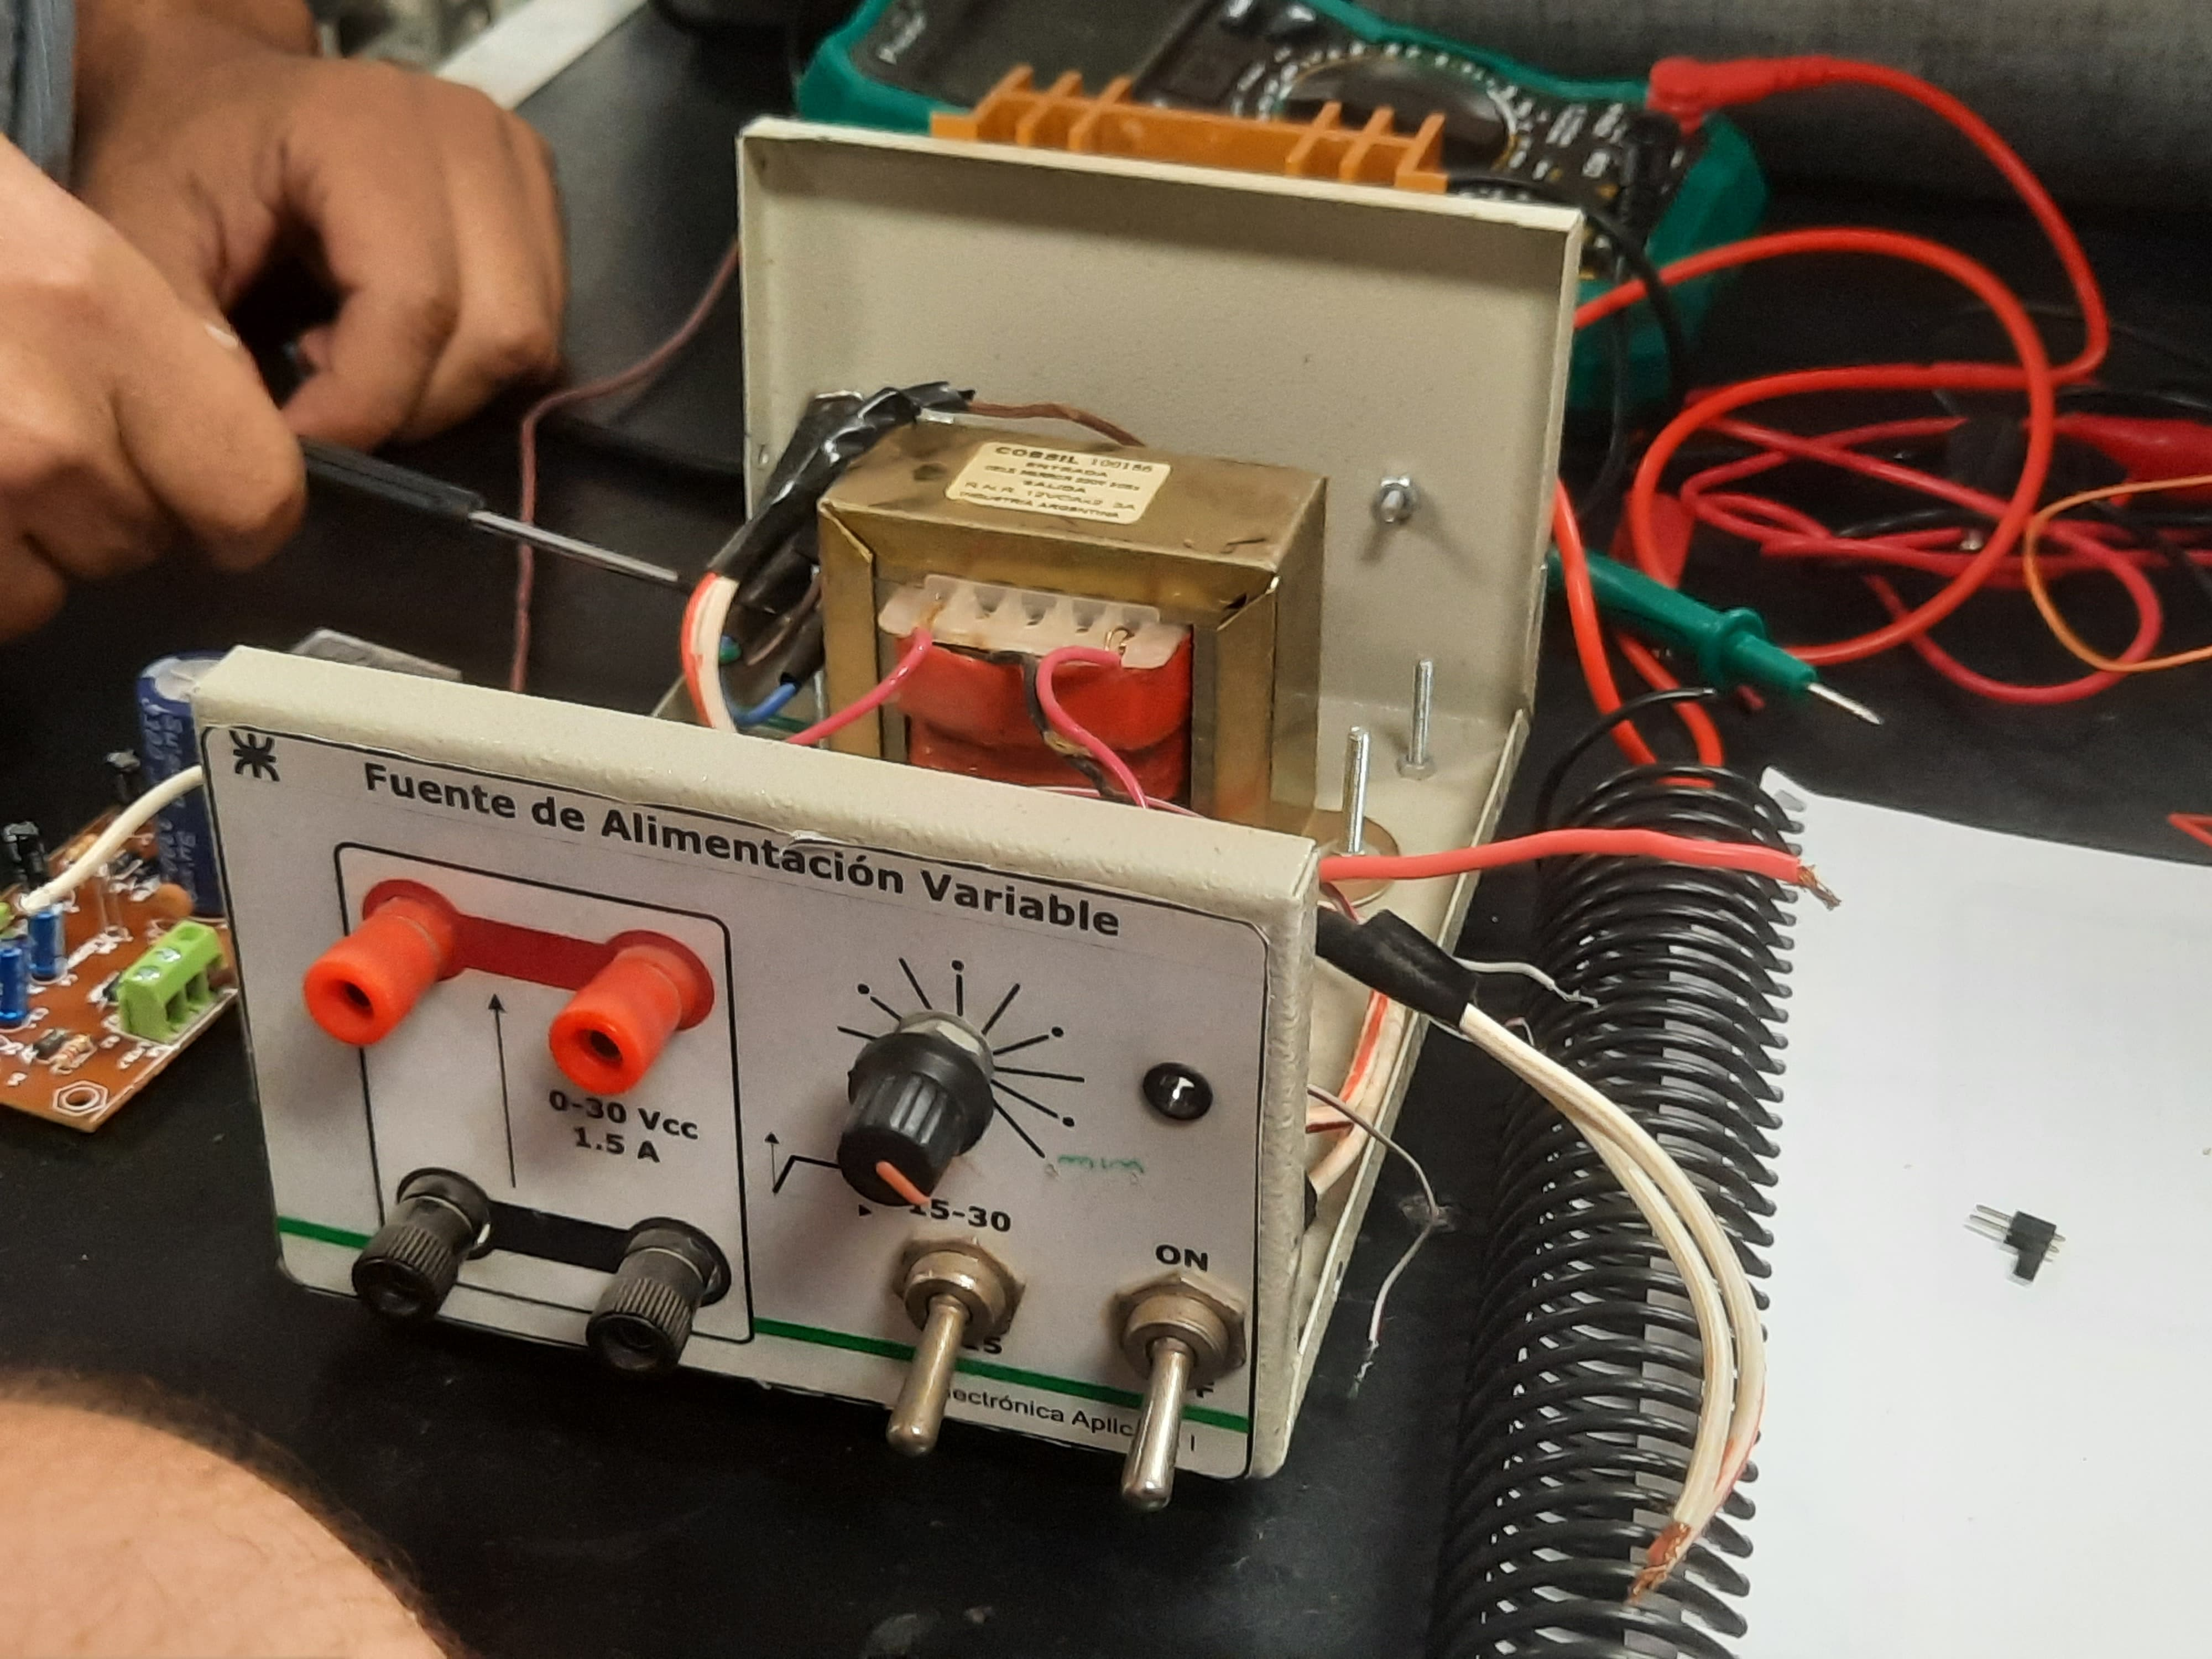
\includegraphics[width=8cm]{./imagenes/portada.jpg}};
    \node at (17cm, -7cm) {\scalebox{5}{\textbf{U}}};
    \node at (17cm, -9cm) {\scalebox{5}{\textbf{T}}};
    \node at (17cm, -11cm) {\scalebox{5}{\textbf{N}}};
    \node at (17cm, -14cm) {\scalebox{5}{\textbf{F}}};
    \node at (17cm, -16cm) {\scalebox{5}{\textbf{R}}};
    \node at (17cm, -18cm) {\scalebox{5}{\textbf{C}}};
    \node at (7.5cm, -14cm) {\scalebox{3}{\textbf{TP N° 2}}};
    \node at (7.5cm, -15cm) {\scalebox{3}{\textbf{Diodos}}};
    \node at (7.5cm, -16cm) {\scalebox{3}{\textbf{Zener y Recortadores}}}; 
    \node at (7.5cm, -23.5cm) {
	\begin{minipage}[c]{12cm}
	    \begin{itemize}
            \raggedright
            \item \fontsize{12}{12}\selectfont \textbf{Autores:} 
                \begin{itemize} \item Gonzalo Ezequiel Filsinger - Leg. 403797  \item Ignacio Ismael Perea - Leg. 106265 \item Mariano Alberto Condori - Leg. \item Marcos Acevedo - Leg.   \end{itemize}
            \item \fontsize{12}{12}\selectfont \textbf{Curso:} 3R1  \\
            \item \fontsize{12}{12}\selectfont \textbf{Asignatura:} Dispositivos Electrónicos.
            \item \fontsize{12}{12}\selectfont \textbf{Institución:} Universidad Tecnológica Nacional - Facultad Regional de Córdoba.
        \end{itemize}
    \end{minipage}};
\end{tikzpicture}
\renewcommand{\headrulewidth}{0.4pt}
\renewcommand{\footrulewidth}{0.4pt}
\definecolor{textoGris}{HTML}{222222}

\fancypagestyle{fancy}{
    \fancyhf{}

    \fancyfoot[R]{[Filsinger G. - Perea I. - Condori M. - Acevedo M.] [\textbf{pág.\ \thepage} de \pageref{LastPage}]}

    \fancyfoot[C]{
        \begin{tikzpicture}[remember picture, overlay]
            \draw[gray!30, line width=0.4pt]
                (0cm, 1cm) -- (0cm, 25cm);
        \end{tikzpicture}
    }

    \fancyhead[L]{
        \begin{tabular}{@{}l@{}}
            \raisebox{-0.5\height}{
\includegraphics[height=0.60in]{./imagenes/logoDepartamentoElectronica.png}}
            \begin{tabular}{@{}l@{}}
                {\color{textoGris}\textbf{Departamento de Ingeniería Electrónica}} \\
                {\color{textoGris}Facultad Regional Córdoba}
            \end{tabular}
        \end{tabular}
    }
}
\titleformat{\section}[hang]{\fontsize{10}{12}\bfseries}{\thesection.}{0.5em}{\underline{#1}}
\titleformat{\subsection}[hang]{\fontsize{10}{11}\bfseries}{\thesubsection.}{0.5em}{#1}
\titleformat{\subsubsection}[hang]{\fontsize{10}{10}\itshape}{\thesubsubsection.}{0.5em}{#1}
\widowpenalty=10000
\clubpenalty=10000
\enlargethispage{-1cm}
\newpage\thispagestyle{empty}\text{}\newpage\newpage\thispagestyle{empty}\setcounter{page}{0}\tableofcontents\newpage\newpage\thispagestyle{empty}\text{}\setcounter{page}{0}

\end{document}